% In this section, describe \emph{what you did}. Roughly speaking, explain what data you worked with, how or from where it was collected, 
% it's structure and size. Explain your analysis, and any specific choices you made in it. Depending on the nature of your project, 
% you may focus more or less on certain aspects. If you collected data yourself, explain the collection process in detail. 
% If you downloaded data from the net, show an exploratory analysis that builds intuition for the data, and shows that you know the data well. 
% If you are doing a custom analysis, explain how it works and why it is the right choice. If you are using a standard tool, 
% it may still help to briefly outline it. Cite relevant works. You can use the \verb|\citep| (whole citation in parenthesis) 
% and \verb|\citet| (only year in parenthesis) commands for this purpose \citep{mackay2003information}.



% SUBSECTION
\subsection{Cardiovascular Diseases data}\label{sec:cardiovascular_data}

In \figurename~\ref{Cardiovascular diseases over time} we can see that Germany has very high incidence and death rate of cardiovascular diseases. 
\begin{figure*}[h]
    \vskip 0.2in
    \centering
    \centerline{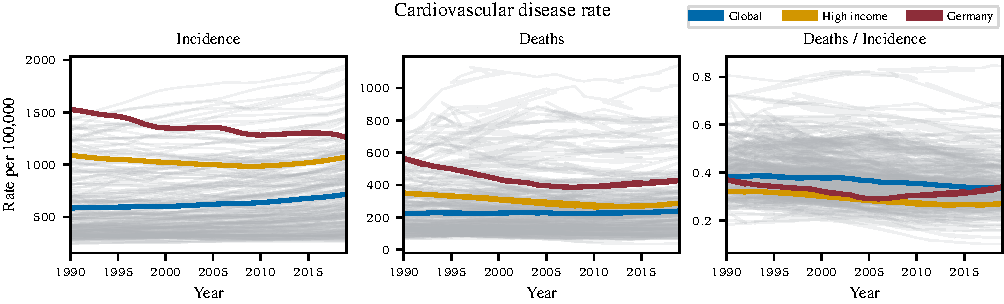
\includegraphics[]{fig/fig_cardiovascular_disease_rate.pdf}}
    \caption{Cardiovascular diseases in the world over time. From left to right: incidence rate, death rate, 
    and the ratio of death rate to incidence rate.}
    \label{Cardiovascular diseases over time}
\end{figure*}


\begin{table}[h]
    \centering
    \caption{Overview of the data sources. The missing data is calculated for the time period from 1990 to 2019.}
    \label{Data overview}
    \begin{tabular}{|c|c|c|c|}
    \hline
    Data source & No. of countries & Missing data\\
    \hline
    Ischemic heart disease & 206 & 0\%\\
    Health expenditure & 50 & 0\%\\
    Fat consumption & 194 & 0\%\\
    Alcohol consumption & 49 & 0\%\\
    Population age & 238 & 0\%\\
    \hline
    \end{tabular}
\end{table}

